

\documentclass[nohyperref]{article}

\usepackage{microtype}
\usepackage{graphicx}
\usepackage{caption}
\usepackage{subcaption}
\usepackage{booktabs} \usepackage{xcolor}
\usepackage{tikz}
\usepackage{pgfplots}
\usepackage{amsmath}
\usepackage{chemarrow}
\usepackage{rotating}
\usepackage{anyfontsize}

\usetikzlibrary{positioning}
\usetikzlibrary{shapes.geometric}
\usetikzlibrary{arrows.meta}
\usetikzlibrary{shapes.misc}
\pgfplotsset{width=\columnwidth, height=4cm, compat=1.9}

\usepackage{hyperref}


\newcommand{\theHalgorithm}{\arabic{algorithm}}



\usepackage[accepted]{icml2023}

\usepackage{amsmath}
\usepackage{amssymb}
\usepackage{mathtools}
\usepackage{amsthm}

\DeclareMathOperator*{\argmax}{arg\,max}
\DeclareMathOperator*{\argmin}{arg\,min}

\usepackage[capitalize,noabbrev]{cleveref}

\theoremstyle{plain}
\newtheorem{theorem}{Theorem}[section]
\newtheorem{proposition}[theorem]{Proposition}
\newtheorem{lemma}[theorem]{Lemma}
\newtheorem{corollary}[theorem]{Corollary}
\theoremstyle{definition}
\newtheorem{definition}[theorem]{Definition}
\newtheorem{assumption}[theorem]{Assumption}
\theoremstyle{remark}
\newtheorem{remark}[theorem]{Remark}

\usepackage[textsize=tiny]{todonotes}


\icmltitlerunning{TR0N: Translator Networks for 0-Shot Plug-and-Play Conditional Generation}

\begin{document}

\twocolumn[
\icmltitle{{\color{violet} TR0N}: {\color{violet}Tr}anslator Networks for {\color{violet}0}-Shot Plug-and-Play Conditional Generatio{\color{violet}n}}





\icmlsetsymbol{equal}{*}

\begin{icmlauthorlist}
\icmlauthor{Zhaoyan Liu}{equal,l6,uoft}
\icmlauthor{No\"{e}l Vouitsis}{equal,l6}
\icmlauthor{Satya Krishna Gorti}{l6}
\icmlauthor{Jimmy Ba}{uoft,vec}
\icmlauthor{Gabriel Loaiza-Ganem}{l6}
\end{icmlauthorlist}

\icmlaffiliation{uoft}{University of Toronto, Toronto, Canada}
\icmlaffiliation{l6}{Layer 6 AI, Toronto, Canada}
\icmlaffiliation{vec}{Vector Institute, Toronto, Canada}

\icmlcorrespondingauthor{Zhaoyan Liu}{zhaoyan@layer6.ai}
\icmlcorrespondingauthor{No\"{e}l Vouitsis}{noel@layer6.ai}
\icmlcorrespondingauthor{Satya Krishna Gorti}{satya@layer6.ai}
\icmlcorrespondingauthor{Jimmy Ba}{jba@cs.toronto.edu}
\icmlcorrespondingauthor{Gabriel Loaiza-Ganem}{gabriel@layer6.ai}

\icmlkeywords{Machine Learning, ICML}

\vskip 0.3in
]





\printAffiliationsAndNotice{\icmlEqualContribution} 

\begin{abstract}
We propose TR0N, a highly general framework to turn pre-trained unconditional generative models, such as GANs and VAEs, into conditional models. The conditioning can be highly arbitrary, and requires only a pre-trained auxiliary model. For example, we show how to turn unconditional models into class-conditional ones with the help of a classifier, and also into text-to-image models by leveraging CLIP. TR0N learns a lightweight stochastic mapping which ``translates'' between the space of conditions and the latent space of the generative model, in such a way that the generated latent corresponds to a data sample satisfying the desired condition. The translated latent samples are then further improved upon through Langevin dynamics, enabling us to obtain higher-quality data samples. TR0N requires no training data nor fine-tuning, 
yet can achieve a zero-shot FID of  on MS-COCO, outperforming competing alternatives not only on this metric, but also in sampling speed -- all while retaining a much higher level of generality. 
Our code is available at \url{https://github.com/layer6ai-labs/tr0n}.
\end{abstract}

\section{Introduction}
Large machine learning models have recently achieved remarkable success across various tasks \citep{brown2020language, jia2021scaling, nichol2021glide, chowdhery2022palm, rombach2022high, yu2022scaling, ramesh2022hierarchical, saharia2022photorealistic, reed2022a}. 
Nonetheless, training such models requires massive computational resources. 
Properly and efficiently leveraging existing large pre-trained models is thus of paramount importance. 
Yet, tractably combining the capabilities of these models in a plug-and-play manner remains a generally open problem. 
Mechanisms to achieve this task should ideally be modular and model-agnostic, such that one can easily swap out a model component for one of its counterparts (e.g.\ interchanging a GAN \citep{goodfellow2014generative} for a VAE \citep{kingma2013auto, rezende2014stochastic}, or swapping CLIP \citep{radford2021learning} for a new state-of-the-art text/image model). 

\begin{figure} [t!]
\centering
\fontsize{7.5}{9}
\selectfont
\begin{tabular}
{p{0.28\linewidth}p{0.28\linewidth}p{0.28\linewidth}}
   \includegraphics[width=2.45cm]{figs/autogan_clip/A_painting_of_a_fox_in_Impressionist_style.png} & \includegraphics[width=2.45cm]{figs/autogan_clip/flaming_portal_to_an_ancient_place.png}
   & \includegraphics[width=2.45cm]{figs/autogan_clip/A_photo_of_a_sunset_over_desert_landscape_with_sand_dunes_and_cacti.png}\\
    A painting of a fox in impressionist style & A photo of a flaming portal to an ancient place rendered in unreal engine &   A photo of a sunset over a desert landscape with sand dunes and cacti\\
   \includegraphics[width=2.45cm]{figs/faces/image_41_Muhammad_Ali.jpg} & 
   \includegraphics[width=2.45cm]{figs/faces/image_1_Tinker_bell.jpg}
   &\includegraphics[width=2.45cm]{figs/faces/image_1_A_man_with_glasses_long_black_hair_with_sideburns_and_a_goatee.jpg}\\
  \hspace{3ex}Muhammad Ali &   \hspace{5ex}Tinker Bell & A man with glasses, long black hair with sideburns and a goatee
\end{tabular}
\vspace{-10pt}
\caption{Images generated by TR0N from corresponding text captions, obtained by finding adequate points on the latent space of a pre-trained GAN. Neither fine-tuning nor training data are used. \textbf{Top row}: BigGAN pre-trained on ImageNet. \textbf{Bottom row}: StyleGAN2 pre-trained on FFHQ.}
\label{fig:fig1}
\vspace{-10pt}
\end{figure} 
\begin{figure*}[th!]
    \centering
    \hspace{-0.75cm}
    \begin{subfigure}[b]{0.18\textwidth}
        \centering
        \resizebox{!}{5cm}{
            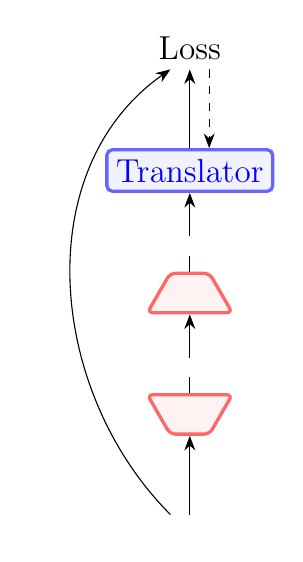
\begin{tikzpicture}[
blue/.style={rectangle, rounded corners=2, draw=blue!60, fill=blue!5, very thick, minimum size=5mm},
red/.style={trapezium, rounded corners=2, trapezium angle=60, draw=red!60, fill=red!5, very thick, minimum size=5mm},
red_inv/.style={trapezium, rounded corners=2, trapezium angle=-60, draw=red!60, fill=red!5, very thick, minimum size=5mm},
font=\large]

\node[anchor=north] (latent) {};
\node[red_inv] (generator) [above=of latent] {\color{red}};
\node[anchor=center] (data) [above=0.2cm of generator] {};
\node[red] (aux) [above=of generator] {\color{red}};
\node[anchor=center] (condition) [above=0.2cm of aux] {};
\node[blue] (translator) [above=of aux] {\color{blue}Translator};
\node[anchor=south] (loss) [above=of translator] {Loss};

\draw[-{Stealth[scale=1.1]}] (latent.north) -- (generator.south);
\draw[-{Stealth[scale=1.1]}] ([xshift=-0.7em]latent.north) to [out=135,in=215] ([xshift=-0.7em]loss.south);
\draw[-] (generator.north) -- (data.south);
\draw[-{Stealth[scale=1.1]}] (data.north) -- (aux.south);
\draw[-] (aux.north) -- (condition.south);
\draw[-{Stealth[scale=1.1]}] (condition.north) -- (translator.south);
\draw[-{Stealth[scale=1.1]}] (translator.north) -- (loss.south);
\draw[dashed, -{Stealth[scale=1.1]}] ([xshift=0.7em]loss.south) -- ([xshift=0.7em]translator.north);

\end{tikzpicture}         }
    \end{subfigure}
    \hspace{-0.5cm}
    \begin{subfigure}[b]{0.18\textwidth}
        \centering
        \resizebox{!}{5cm}{
            \begin{tikzpicture}[
blue/.style={rectangle, rounded corners=2, draw=blue!60, fill=blue!5, ultra thick, minimum size=5mm},
red/.style={rectangle, rounded corners=2, draw=red!60, fill=red!5, ultra thick, minimum size=5mm},
font=\Large]
\makeatletter
\newcommand{\xdashrightarrow}[2][]{\ext@arrow 0359\rightarrowfill@@{#1}{#2}}
\def\rightarrowfill@@{\arrowfill@@\relax\relbar\chemarrow}
\def\arrowfill@@#1#2#3#4{#4#2}
\makeatother

\matrix [draw] at (0,0) (legend) {
  \node [red,label={[label distance=0.35cm]right: Frozen weights}] {}; \\
  \0.075cm]
  \node [label=right:Gradient update] {\Large}; \\
};

\node[anchor=center] (tron_left) [above=2.5cm of legend] {\LARGE \hspace{-15ex} {\textbf{TR0N}}};
\node[anchor=center] (tron_right) [above=2.5cm of legend] {\LARGE \hspace{15ex} {\textbf{TR0N}}};
\node[anchor=center] (title_left) [above=1.75cm of legend] {\LARGE \hspace{-15ex} {\textbf{training}}};
\node[anchor=center] (title_right) [above=1.75cm of legend] {\LARGE \hspace{15ex} {\textbf{sampling}}};



\draw[-] ([yshift=-3.5cm]legend.south) -- ([yshift=-0.25cm]legend.south);
\draw[-] ([yshift=3.5cm]legend.north) -- ([yshift=0.25cm]legend.north);
\end{tikzpicture}         }
    \end{subfigure}
    \hspace{0.5cm}
    \begin{subfigure}[b]{0.62\textwidth}
        \centering
        \resizebox{!}{5cm}{
            \begin{tikzpicture}[
red_rec/.style={rectangle, rounded corners=2, draw=red!60, fill=red!5, very thick, minimum size=5mm},
red/.style={trapezium, rounded corners=2, trapezium angle=60, draw=red!60, fill=red!5, very thick, minimum size=5mm},
red_inv/.style={trapezium, rounded corners=2, trapezium angle=-60, draw=red!60, fill=red!5, very thick, minimum size=5mm},
red_90/.style={trapezium, rounded corners=2, rotate=-90, trapezium angle=60, draw=red!60, fill=red!5, very thick, minimum size=5mm},
font=\large]

\node[anchor=center] (condition) {A sheepdog in sketch style};
\node[anchor=center] (c) [above=0.25cm of condition] {};
\node[red_rec] (translator) [above=0.35cm of c] {\color{red}Translator};
\node[anchor=center] (latent0) [above=0.65cm of translator] {};
\node[red_90] (generator0) [below left=-0.02cm and 0.35cm of latent0] {\rotatebox{90}{\color{red}}};
\node[inner sep=0pt] (sheepdog0) [left=1.3cm of latent0]
    {\includegraphics[height=2cm]{figs/sheepdog_step0.jpg}};
\node[anchor=center] (loss0) [above=2.75cm of latent0] {};
\node[anchor=center] (break1) [above right=1.75cm and 1.1cm of latent0] {};
\node[anchor=center] (break2) [below=0.5cm of break1] {};
\node[anchor=center] (break3) [below=1.92cm of break1] {};
\node[anchor=center] (latent1) [right=2.5cm of latent0] {};
\node[anchor=center] (loss1) [above=2.75cm of latent1] {};
\node[anchor=center] (latent2) [right=2.5cm of latent1] {};
\node[anchor=center] (ellipsis) [right=0.9cm of latent2] {\ldots};
\node[anchor=center] (latentT) [right=2.5cm of latent2] {};
\node[red_inv] (generatorT) [above=0.35cm of latentT] {\color{red}};
\node[inner sep=0pt] (sheepdogT) [above=0.35cm of generatorT]
    {\setlength{\fboxsep}{0pt}\fbox{\includegraphics[height=2cm]{figs/sheepdog_stepT.jpg}}};

\draw[-] (condition.north) -- (c.south);
\draw[-] (c.east) to [out=0,in=270] (break3.south);
\draw[-] (break3.north) -- (break2.south);
\draw[-] (break2.north) -- (break1.south);
\draw[-{Stealth[scale=1.1]}] (break1.south) to [out=90,in=345] ([xshift=0.70em]loss0.south);
\draw[-{Stealth[scale=1.1]}] (break1.south) to [out=90,in=195] ([xshift=-0.35em]loss1.south);
\draw[-{Stealth[scale=1.1]}] (c.north) -- (translator.south);
\draw[-] (translator.north) -- (latent0.south);
\draw[-{Stealth[scale=1.1]}] (latent0.north) -- (loss0.south);
\draw[-{Stealth[scale=1.1]}] (latent0.west) -- (generator0.north);
\draw[-{Stealth[scale=1.1]}] (generator0.south) -- (sheepdog0.east);
\draw[dashed, -{Stealth[scale=1.1]}] ([xshift=0.35em]loss0.south) -- ([xshift=-0.15em, yshift=0.35em]latent1.west);
\draw[-{Stealth[scale=1.1]}] (latent0.east) -- (latent1.west);
\draw[-{Stealth[scale=1.1]}] (latent1.north) -- (loss1.south);
\draw[dashed, -{Stealth[scale=1.1]}] ([xshift=0.35em]loss1.south) -- ([xshift=-0.15em, yshift=0.35em]latent2.west);
\draw[-{Stealth[scale=1.1]}] (latent1.east) -- (latent2.west);
\draw[-{Stealth[scale=1.1]}] (latent2.east) -- ([xshift=-5em]latentT.west);
\draw[-{Stealth[scale=1.1]}] ([xshift=5.15em]latent2.east) -- (latentT.west);
\draw[-{Stealth[scale=1.1]}] (latentT.north) -- (generatorT.south);
\draw[-{Stealth[scale=1.1]}] (generatorT.north) -- (sheepdogT.south);
\end{tikzpicture}         }
    \end{subfigure}   
    \caption{\textbf{Left panel}: The stochastic translator network learns to recover  from . \textbf{Right panel}: The (stochastic) output  of the trained translator -- which is such that  ``roughly satisfies'' condition  -- initializes Langevin dynamics over  which further improves the sample so as to better match . In the depicted example,  is a GAN trained on ImageNet,  the CLIP image encoder,  the CLIP text embedding corresponding to the given text prompt, and  the negative cosine similarity between  and .}
\label{fig:tron}
\end{figure*}

In this work, we study conditional generation through the lens of combining pre-trained models. 
Conditional generative models aim to learn a conditional distribution of data given some conditioning variable . 
They are typically trained from scratch on pairs of data with corresponding  (e.g.\ images , with corresponding class labels or text prompts fed through a language model ) \citep{mirza2014conditional, sohn2015learning}. Our goal is to take an arbitrary pre-trained unconditional pushforward generative model \citep{salmona2022can, ross2022neural} --  i.e.\ a model  which transforms latent variables  sampled from a prior  to data samples  -- and turn it into a conditional model. To this end, we propose TR0N, a highly general framework to make pre-trained unconditional generative models conditional. TR0N assumes access to a pre-trained auxiliary model  that maps each data point  to its corresponding condition , e.g.\  could be a classifier, or a CLIP encoder. TR0N also assumes access to a function  such that latents  for which  ``better satisfies'' a condition  are assigned smaller values. Using this function, for a given , TR0N performs  steps of gradient minimization of  over  to find latents that, after applying , will generate desired conditional data samples.

However, we show that na\"ively initializing the optimization of  is highly suboptimal. With this in mind, TR0N starts by learning a network that we use to better initialize the optimization process. We refer to this network as the translator network since it ``translates" from a condition  to a corresponding latent  such that  is small, essentially amortizing the optimization problem. Importantly, the translator network is trained \emph{without fine-tuning  or  nor using a provided dataset}. In this sense, TR0N is a zero-shot method wherein the only trainable component is a lightweight translator network. Importantly, TR0N avoids the highly expensive training of a conditional model from scratch and is model-agnostic: we can use any  and any , which also makes it straightforward to update any of these components whenever a newer state-of-the-art version becomes available. We outline the procedure to train the translator network on the left panel of \autoref{fig:tron}.

Once the translator network is trained, we use its output to initialize the optimization of . This reclaims any performance lost due to the amortization gap \citep{cremer2018inference,kim2018semi}, resulting in better local optima and faster convergence than na\"ive initialization. In reality, TR0N is a stochastic method: the translator network is a conditional distribution  that assigns high density to latents  such that  is small, and we add noise during the gradient optimization of , which allows us to interpret TR0N as sampling with Langevin dynamics \citep{welling2011bayesian} using an efficient initialization scheme. We exemplify how to sample with TR0N on the right panel of \autoref{fig:tron}.

Our contributions are:  introducing translator networks and a particularly efficient parameterization of them, allowing for various ways to initialize Langevin dynamics;  framing TR0N as a highly general framework, whereas previous related works mostly focus on a single task with specific choices of  and ; and  showing that TR0N empirically outperforms competing alternatives across tasks in image quality and computational tractability, while producing diverse samples; and that it can achieve an FID \citep{Heusel2017GANsTB} of  on MS-COCO \citep{lin2014microsoft}.
 
\section{Background}
\paragraph{Joint text/image models} In this work, we leverage pre-trained joint text/image models as a particular choice for both the auxiliary model  and to construct , enabling TR0N to be conditioned on either free-form text prompts or on image semantics. 
Recent joint text/image models such as CLIP learn a joint representation space  for images and texts. 
CLIP includes an image encoder  and a text encoder , where  is the space of images and  is the space of text prompts, which are trained in such a way that images and texts that are semantically aligned are mapped to similar representations. 
More specifically, CLIP is such that the negative cosine similarity  is small for semantically aligned image/text pairs , and large for semantically unaligned pairs, where .


\paragraph{Pushforward models} We use the term \emph{pushforward model} to refer to any generative model whose samples  can be obtained as , where  is a latent variable sampled from some (typically not trainable) prior , and  is a neural network. 
Many models fall into this category, including generative adversarial networks (GANs), variational autoencoders (VAEs), normalizing flows \citep{dinh2016density, durkan2019neural} and variants thereof \citep{brehmer2020flows, caterini2021rectangular, ross2021tractable}, and more \citep{tolstikhin2017wasserstein,loaiza2022diagnosing}. We focus on GANs and VAEs since they use a low-dimensional latent space , which will later make the translator network's task easier. Our main goal is to turn a pre-trained unconditional pushforward model  into a conditional model .

\paragraph{EBMs and Langevin dynamics} We will later formalize the goal of TR0N as sampling from a distribution  defined only up to proportionality, i.e.\ , where  is called the energy function, and the hyperparameter  controls the degree to which small values of  correspond to large values of , and vice-versa. We hereafter refer to this formulation as an energy-based model (EBM). While the energy function in EBMs is typically learnable \citep{xie2016theory,du2019implicit}, in our work we define and fix an energy function that allows us to enforce the requirement that ``applying  to a sample from  satisfies condition ''. 
Langevin dynamics is a method that allows us to sample from EBMs by constructing a Markov chain  given by

where the sequence  is a hyperparameter, and . Under mild conditions and by sending  to  at an appropriate rate, 
the limiting distribution of this Markov chain as  is . 
Langevin dynamics can be interpreted as gradient descent on  with added noise, and has been successfully applied to sample and train deep EBMs, where in practice it is common to deviate from theory and set  for all  (i.e.\ a single scalar hyperparameter  is used) for improved empirical performance. 
Also, while in theory convergence does not depend upon the starting point , in practice this choice can greatly speed up convergence \citep{hinton2002training, nijkamp2020anatomy, yoon2021autoencoding}, just as with gradient descent \citep{boyd2004convex, glorot2010understanding}.
 
\section{TR0N}
\subsection{Plug-and-play components of TR0N}

TR0N requires three key components to ensure that it can operate as a plug-and-play framework. First, TR0N takes an arbitrary pre-trained pushforward model . 
TR0N also assumes access to a pre-trained auxiliary model  that maps data to its corresponding condition. For example, if our goal is to condition on class labels,  would be a classifier, and  the space of probability vectors of appropriate length. If we aim to condition on text,  could be given by the CLIP image encoder  -- although we will see later that a different choice of  led us to improved empirical performance in this setting -- and  the latent space of CLIP, .  
The final component of TR0N is a function  which measures how much  satisfies condition , an intuitive choice being 

where  measures discrepancy between conditions, for example: when  is a classifier,  could be the categorical cross entropy; and when  is the image encoder from CLIP,  could be the negative cosine similarity, . However, other choices of  are possible, as we will show in our experiments.

\subsection{Overview of TR0N}

\paragraph{Translator networks} TR0N uses the aforementioned components to train the translator network which, given , aims to output a  with small . This can be intuitively understood as amortizing the minimization of  with a neural network so as to not have to run a minimizer from scratch for every . Since there can be many latents  for which  satisfies  (i.e.  is small), we propose to have the translator be a distribution , parameterized by . This way, the translator can assign high density to all the latents  such that  is small. We will detail how we instantiate  with a neural network in \autoref{sec:gmm}, but highlight that any choice of conditional density is valid. Importantly, since we have access to the unconditional model , we can generate synthetic data  with ; and since we have access to , we can obtain the condition corresponding to , namely . Together, this means that the translator can be trained through maximum likelihood \emph{without the need for a provided training dataset}, through

We summarize the above objective in Algorithm \ref{alg:training}.

\begin{algorithm}[t]
   \caption{TR0N training}
   \label{alg:training}
\begin{algorithmic}
   \STATE {\bfseries Input:} , , , , and batch size 
   \WHILE{not converged}
   \STATE Sample  for 
   \STATE  for 
   \STATE 
   \STATE Use  to update , e.g.\ with ADAM \citep{kingma2015adam}
   \ENDWHILE
\end{algorithmic}
\end{algorithm}

\paragraph{Error correction} The translator is trained to stochastically recover  from , so that intuitively it places high densities on latents which have low  values. Yet, the translator is not directly trained to minimize , and thus having an error correction step, over which  is explicitly optimized, is beneficial to further improve its output. Thus, for a given , we run  steps of gradient descent on  over , which we initialize with the help of the translator. Initializing optimization with  rather than na\"ively (e.g\ Gaussian noise) significantly speeds up convergence, and as we will see in our experiments, can also lead to better local optima. Importantly, we can use the translator in various ways to initialize optimization. For example, we can sample  times from , and use the sample with the lowest  value (which would be impossible if the translator was deterministic). We will detail another way to leverage the translator network to initialize optimization in \autoref{sec:gmm}. In practice, we add Gaussian noise to gradient descent. Together with the stochasticity of the translator, this ensures diverse samples. Lastly, we transform the final latent, , through  to obtain a conditional sample from TR0N. We summarize this procedure in Algorithm \ref{alg:sampling}.


\subsection{TR0N as an EBM sampler}

TR0N can be formalized as sampling from an EBM with Langevin dynamics. Defining the distribution , which we call the \emph{conditional prior}, as , Algorithm \ref{alg:sampling} uses Langevin dynamics \eqref{eq:langevin_dynamics} to sample from , initialized with the help of . Thus, TR0N can be interpreted as a sampling algorithm for the conditional pushforward model . Again,  remains fixed throughout, and conditioning is achieved only through the prior . 
In this view, the translator network  can be understood as a rough approximation to , as both of these distributions assign large densities to latents  for which  is small. This is precisely why the translator provides a good initialization for Langevin dynamics: the more  ``comes from '', the faster \eqref{eq:langevin_dynamics} will converge.

\paragraph{Why maximum-likelihood?} If our goal is for the translator to be close to the conditional prior, i.e.\ , then a natural question is why train the translator through \eqref{eq:ml}, which does not involve , rather than by minimizing some discrepancy between these two distributions? The answer is that, since the target  is specified only up to proportionality and true samples from it are not readily available (better sampling from  is in fact what we designed TR0N to achieve), minimizing commonly-used discrepancies such as the KL divergence or the Wasserstein distance is not tractable. The only discrepancy we are aware of that could be used in this setting is the Stein discrepancy, which has also been used to train EBMs \citep{grathwohl2020learning}. However, in preliminary experiments we observed very poor results by attempting to minimize this discrepancy. In contrast, the maximum-likelihood objective \eqref{eq:ml} is straightforward to optimize, and obtained strong empirical performance in our experiments.

\begin{algorithm}[t]
   \caption{TR0N sampling}
   \label{alg:sampling}
\begin{algorithmic}
   \STATE {\bfseries Input:} , , , , , , , 
   \STATE {\bfseries Output:} 
   \STATE Initialize  with , e.g.\  for , and 
   \FOR{ {\bfseries to} }
   \STATE Sample 
   \STATE 
   \ENDFOR
\end{algorithmic}
\end{algorithm}


\subsection{GMMs to parameterize translator networks}\label{sec:gmm}

While clearly any choice of conditional density model  can be used in TR0N, we choose a Gaussian mixture model (GMM), as it has several advantages that we will discuss shortly. More specifically, we use a neural network, parameterized by , which maps conditions  to the mean  and weight  parameters of a Gaussian mixture, i.e.\

where  has positive entries which add up to one (enforced with a softmax), and , i.e.\  is learnable. 
We use a simple multilayer perceptron with multiple heads to parameterize this neural network.

Our GMM choice for the stochastic translator has four important benefits:  It is a very lightweight model, and thus achieves our goal of being much more tractable to train than any of the pre-trained components  and , which we once again highlight remain fixed throughout.  Sampling from a GMM is very straightforward and can be done very quickly.  Empirically, we found that using more complicated density models  such as normalizing flows did not result in improved performance. We hypothesize that, since Langevin dynamics acts as an error correction step,  just needs to approximate, rather than perfectly recover, .  Finally, taking  as a GMM allows using the translator to initialize Langevin dynamics in ways that are not straightforward to extend to a non-GMM setting. In particular, we found that sometimes (when diversity is not as paramount), rather than initializing \eqref{eq:langevin_dynamics} as described in Algorithm \ref{alg:sampling}, better performance could be achieved by directly using the GMM parameters. That is, we initialize at the GMM mean, . Note that the mean of more complex distributions might not be so easily computable. Further, we found that when initializing this way, optimizing the weights and means directly yielded better performance, i.e\ we write  as , and perform Langevin dynamics as

where ,  for , and the size of  is appropriately changed from \eqref{eq:langevin_dynamics}.

\subsection{TR0N for Bayesian inference}\label{sec:bayes}

In some settings, the auxiliary model  might provide a probabilistic model . For example, when  is a classifier, .\footnote{We slightly abuse notation here and use  interchangeably as either a one-hot vector, or as the corresponding integer index.}  Combined with the pushforward model, this provides a latent/data/condition joint distribution , where  denotes a point mass on  at . For Bayesian inference, it might be of interest to sample from the corresponding posterior , which is equivalent to sampling from  and transforming the result through . That is, in this scenario, the conditional prior  is a proper posterior distribution of latents given a condition. TR0N can sample from this posterior by using specific choices of  and . While these choices provide a probabilistically principled way of combining  and  into a conditional model, we find that non-Bayesian choices obtain stronger empirical results. We nonetheless believe that TR0N being compatible with Bayesian inference is worth highlighting. Due to space constraints, we include additional details in Appendix \ref{app:bayes}.

%
 
\section{Related Work}
\begin{figure*}[t!]
    \centering
    \includegraphics[width=0.2375\linewidth]{figs/NVAE_CIFAR10/unconditional_nvae_fid_41_7.png} \hspace{0.05cm}
    \includegraphics[width=0.2375\linewidth]{figs/NVAE_CIFAR10/conditional_nvae_fid18_top10.png}
    \hspace{0.05cm}
    \includegraphics[width=0.2375\linewidth]{figs/autogan_classifier/autogan_unconditional.png}
    \hspace{0.05cm}
    \includegraphics[width=0.2375\linewidth]{figs/autogan_classifier/trans_gmm_conditional_autogan.png}
    \caption{Samples from NVAE (\textbf{first panel}), TR0N:NVAE+ResNet50 (\textbf{second panel}), AutoGAN (\textbf{third panel}), and TR0N:AutoGAN+ResNet50 (\textbf{fourth panel}). Rows on the second and fourth panels correspond to classes: TR0N  learns to diversely sample in a class-conditional way, while retaining the image quality of the underlying unconditional model. Best viewed while zoomed-in.}
    \label{fig:cifar_conditioning}
\end{figure*}

Several methods aim to obtain a conditional generative model by combining pre-trained models, although none of them shares all of the advantages of TR0N. 
Notably, almost all the works we discuss below are shown to work for a single task, unlike TR0N which is widely applicable.

\paragraph{Non-zero-shot methods} \citet{Zhou2021TowardsLT} and \citet{Wang2022CLIPGENLT} leverage CLIP to train text-to-image models without text data, but unlike TR0N, still require a training dataset of images and relatively longer training times. \citet{wang2022traditional} propose a method to turn a classifier into a conditional generative model which also requires training data to train a masked autoencoder. \citet{nie2021controllable} condition GANs through a similar EBM as us, but use data to train , do not condition on text, and do not use translator networks. \citet{zhang2023adding} add conditioning to pre-trained diffusion models \citep{ho2020denoising}, but require training data to do so.

\paragraph{Deterministic optimization} The works of \citet{nguyen2016synthesizing}, \citet{liu2021fusedream}, \citet{patashnik2021styleclip}, and \citet{li2022composing} can be thought of as deterministic versions of our EBM, where rather than sampling from , the energy  is directly minimized over . These methods do not account for the fact that there can be many latents  such that  satisfies condition , and thus can be less diverse than TR0N. Additionally, these methods do not have a translator network, and with the exception of FuseDream \citep{liu2021fusedream}, na\"ively initialize optimization, resulting in reduced empirical performance and needing more gradient steps for optimization to converge. We also note that FuseDream's initialization scheme -- which we detail in Appendix \ref{app:exp_details} for completeness -- requires many forward passes through  and , and remains much more computationally demanding than TR0N's.

\paragraph{Stochastic methods} \citet{ansari2021refining} apply Langevin dynamics on the latent space of a GAN, but do so to iteratively refine its samples, rather than for conditional sampling. \citet{nguyen2017plug} use a similar EBM to ours, but do not use a translator network and initialize Langevin dynamics na\"{i}vely, once again resulting in significantly decreased empirical performance as compared to TR0N. \citet{promptgen2022} also define a similar EBM to ours, which is approximated with a normalizing flow for each different , meaning that a different model has to be trained for each condition, resulting in a method that is far less scalable than TR0N. Finally, \citet{Pinkney2022clip2latent} propose clip2latent, which can be understood as using a diffusion model instead of a GMM as the translator network, making clip2latent more expensive to train than TR0N. Importantly, they perform no error correction step whatsoever, and thus do not leverage important information contained in the gradient of .
 
\section{Experiments}
All our experimental details -- including which translator-based initialization we used for each experiment -- are provided in Appendix \ref{app:exp_details}.

\subsection{Conditioning on class labels}

We demonstrate TR0N's ability to make an unconditional model on CIFAR-10 \citep{krizhevsky2009learning} into a class-conditional one. To highlight the flexibile plug-and-play nature of TR0N, we use two different pushforward models : an NVAE \citep{Vahdat2020NVAEAD}, and an AutoGAN \citep{Gong2019AutoGANNA} -- we use this somewhat non-standard choice of GAN since most publicly available GANs pre-trained on CIFAR-10 are class-conditional. 
Here,  is the space of probability vectors of length , we take  as a ResNet50 classifier \cite{He2015DeepRL}, and use  as in \eqref{eq:score} with  given by the cross-entropy loss, .

\autoref{fig:cifar_conditioning} shows qualitative results: we can see that, for both pushforward models, TR0N not only obtains samples from each of the 10 classes, but that it achieves this without sacrificing neither image quality nor diversity. 

We also make quantitative comparisons between each unconditional model (i.e.\ NVAE and AutoGAN) and the resulting conditional models provided by TR0N. To make the comparison equitable, we sample unconditionally from TR0N models by first sampling one of the  classes uniformly at random, and then sampling from the corresponding conditional. Results are shown in \autoref{table:cifar-table}, by measuring image quality and diversity through both the FID score and the inception score \citep{salimans2016improved}, and the quality of conditioning through the average probability that the ResNet50 assigns to the intended class of TR0N samples. TR0N not only makes the models conditional as these probabilities are very close to , especially for the AutoGAN-based model, but it also improves their FID and inception scores (IS): TR0N leverages the classifier  not only to make a conditional model, but also to improve upon its underlying pre-trained pushforward model.

\begin{figure*} [h!]
\hspace*{-0.2cm}
\centering
\fontsize{8.5}{10}
\selectfont
\begin{tabular}
{p{0.145\linewidth}p{0.145\linewidth}p{0.145\linewidth}p{0.145\linewidth}p{0.145\linewidth}p{0.145\linewidth}}
   \includegraphics[width=2.6cm]{figs/TR0N_diversity/insect_seed_1_0.png} & \hspace{-0.25cm}\includegraphics[width=2.6cm]{figs/TR0N_diversity/insect_seed_1_1.png} &\includegraphics[width=2.6cm]{figs/TR0N_diversity/beach_3_9.png} & \hspace{-0.25cm}\includegraphics[width=2.6cm]{figs/TR0N_diversity/beach_200_2.png} & \includegraphics[width=2.6cm]{figs/TR0N_diversity/gothic_church_seed_1_0.png}
   & \hspace{-0.25cm}\includegraphics[width=2.6cm]{figs/TR0N_diversity/gothic_church_seed_1_1.png}\-0.3cm]
    \caption{Comparisons between TR0N:BigGAN+CLIP and FuseDream on MS-COCO as a function of time required to generate a sample. \textbf{Top panel}: FID score (in log scale), lower is better. \textbf{Bottom panel}: augmented CLIP score, higher is better.}
    \label{fig:fid_vs_iters}
    \vskip -0.1in
\end{figure}

\begin{figure*} [h!]
\newcommand{\centered}[1]{\begin{tabular}{c} #1 \-0.25cm] 
\end{tabular}
\caption{Comparison between TR0N:StyleGAN2+CLIP (\textbf{top row}) and clip2latent (\textbf{bottom row}). Numbers above each image correspond to average augmented CLIP score (higher is better) plus/minus standard error over  samples from the given caption. Thanks to the error correction step, TR0N better semantically matches the input text in its generated images than clip2latent.}
\label{fig:stylegan_faces}
\end{figure*} 
We compare TR0N against FuseDream on the MS-COCO dataset, which contains text/image pairs. For each text, we generate a corresponding image with both methods, and then compute both the FID and augmented CLIP score. Results are displayed in \autoref{fig:fid_vs_iters} for various computational budgets (the higher the budget, the bigger , i.e.\ the longer Langevin dynamics is iterated for). 
As a consequence of FuseDream's expensive initialization scheme, TR0N can achieve similar performance much faster. This is true for our first choice of , where TR0N uses the same components as FuseDream (red vs orange lines), emphasizing once again the relevance of the translator, as also evidenced by the light blue lines in \autoref{fig:fid_vs_iters}, which correspond to TR0N with no translator (or equivalently, FuseDream with na\"ive initialization). 
It is also true for our second choice of  (with a caption model), which allows TR0N to not only be faster than FuseDream (which cannot incorporate this  as it has no translator), but also outperform it (blue vs orange lines). 
We once again perform ablations over different design choices of the translator, which we include in Appendix \ref{app:extra_exps}.

\autoref{fig:fig1} and \autoref{fig:TR0N_diversity} show text-to-image samples from TR0N. Although BigGAN was trained on ImageNet and remains fixed throughout, the images that TR0N manages to produce from it using text prompts are highly out-of-distribution for this dataset: TR0N's ability to efficiently leverage CLIP to explore the GAN's latent space  is noteworthy. We include additional samples in Appendix \ref{app:extra_exps}, showing both how images evolve throughout Langevin dynamics, and failure cases of TR0N.

By using the same  and version of CLIP as FuseDream, the previous experiments show that TR0N outperforms it thanks to its methodology, rather than an improved choice of networks.
Yet, these networks can be improved. To further strengthen TR0N,  we upgrade:  to a StyleGAN-XL \citep{sauer2022stylegan} -- also pre-trained on ImageNet, CLIP to its LAION2B \citep{schuhmann2022laionb} version, and the caption model to BLIP-2 \citep{li2023blip} (using BLIP-2 instead of BLIP as in other experiments again highlights the plug-and-play nature of TR0N). \autoref{table:ms-coco-fid} shows quantitative results, where we can see that these updates significantly boost the performance of TR0N, to the point of making it competitive with very large models requiring text/image data and much more compute to train. While this StyleGAN-XL-based version of TR0N achieves particularly strong results on MS-COCO in terms of FID, we find that the images it produces are not consistently better, visually, than those from the BigGAN-based model. Samples and further discussion can be found in Appendix \ref{app:extra_exps}.


\paragraph{Facial images} To further highlight the wide applicability of TR0N, we show it can be used for other text-to-image tasks. We now use a StyleGAN2 \citep{Karras2019stylegan2} and an NVAE as , both pre-trained on FFHQ \citep{karras2019style}. We use CLIP's image encoder  as  (we do not use a caption model here as the descriptions of faces it outputs are too generic to be useful), and use the negative augmented clip score  as . We compare against clip2latent, which uses the same setup with the StyleGAN2, but with a diffusion model instead of a GMM as a translator network, and no error correction procedure.

\begin{table}[t]
\vskip -0.1in
\caption{FID score on MS-COCO. The top part of the table shows models trained directly for text-to-image generation using paired text/image data (these are sometimes called zero-shot as they were not trained on MS-COCO, but are not zero-shot in the same way as TR0N). The bottom part shows zero-shot methods that require only pre-trained models and no provided dataset.}
\begin{center}
\scalebox{0.76}{
\begin{tabular}{lcr}
\toprule
Model & FID  \\
\midrule
DALL-E \citep{ramesh2021zero} & \\
StyleGAN-T \citep{sauer2023stylegan} & \\
Latent Diffusion \citep{rombach2022high} & \\
GLIDE \citep{nichol2021glide} & \\
DALL-E 2 \citep{ramesh2022hierarchical} & \\
Imagen \citep{saharia2022photorealistic} & \\
Parti \citep{yu2022scaling} & \\
\midrule
FuseDream \citep{liu2021fusedream} &  \\
TR0N:BigGAN+CLIP (BLIP) &  \\
TR0N:StyleGAN-XL+LAION2BCLIP (BLIP-2) & \\
\bottomrule
\multicolumn{2}{l}{\small \hspace{5pt}  Score as reported by the authors, not computed by us.}\\
\multicolumn{2}{l}{\small \hspace{5pt}  \citet{liu2021fusedream} report an FID of  since they use ADAM instead of}\\
\multicolumn{2}{l}{\small \hspace{12pt} Langevin dynamics.}
\end{tabular}
}
\end{center}
\label{table:ms-coco-fid}
\vskip -0.2in
\end{table}

\begin{figure*} [h!]
\newcommand{\centered}[1]{\begin{tabular}{c}  \-1.6cm] #1 \end{tabular}}
\renewcommand\fbox{\fcolorbox{black!15!red}{white}}
\centering
\hspace*{-0.2cm}
\begin{tabular}
{ccccc}
   \hspace{-0.1cm}\centered{{\setlength{\fboxsep}{0pt}\setlength{\fboxrule}{0.075cm}\fbox{\includegraphics[width=1.35cm]{figs/image_var/sea.jpg}}}} & \hspace{-0.64cm}\includegraphics[width=1.5cm]{figs/image_var/sea_1.jpg} & \centered{{\setlength{\fboxsep}{0pt}\setlength{\fboxrule}{0.075cm}\fbox{\includegraphics[width=1.35cm]{figs/image_var/bear.jpg}}}} & \hspace{-0.64cm}\includegraphics[width=1.5cm]{figs/image_var/bear_1.jpg} & \centeredi{\includegraphics[width=9.5cm]{figs/image_var/interp1.jpg}} \\label{eq:bayes}
    E_{\text{Bayes}}(z,c) = -\log p(z) - \log p(c|x=G(z)).
\label{eq:bayes_prime}
    E_{\text{Bayes}}'(z,c) = -\beta_1 \log p(z) - \beta_2 \log p(c|x=G(z)),
\label{app_eq:l2}
    \theta^* = \argmin_\theta \mathbb{E}_{p(z)}\left[\Vert S_\theta(f(G(z))) - z\Vert_2^2\right].
\label{eq:nvae_prior}
    p(z') = p(z_0) \displaystyle \prod_{\ell=1}^L p(z_\ell|z_{\ell - 1}),
\label{eq:nvae_z_det}
    z_\ell = g_\ell(z_{\ell-1}) \text{ for }\ell=1,\dots,\ell^*,
\label{eq:nvae_z_rand}
    z_\ell|z_{\ell-1} \sim p(z_\ell|z_{\ell-1}) \text{ for }\ell=\ell^*+1,\dots,L.

    \theta^* = \argmin_\theta \mathbb{E}_{p(z)}\left[-\log q_\theta \left(z|c=f(G(z))+\gamma \epsilon \right)\right],
-0.05cm]
   A photo of a snowy valley \-0.05cm]
   A light shining in the night \-0.05cm]
   A crayon drawing of a space elevator
\end{tabular}
\caption{Evolution of samples throughout Langevin dynamics for our TR0N:BigGAN+CLIP (BLIP) model. Each row shows  for increasing values of  for the corresponding text prompt.}
\label{fig:langevin_evolution}
\end{figure*}







\autoref{fig:langevin_evolution} shows how samples evolve throughout Langevin dynamics. We can see that the output of the translator provides a sensible initialization, and that image quality improves throughout Langevin dynamics. Not surprisingly, the output of the translator more closely matches the given text prompt for in-distribution prompts (e.g.\ ``A photo of a snowy valley'') than for out-of-distribution prompts (e.g.\ ``A crayon drawing of a space elevator''), although the initialization remains useful for all situations.

\autoref{fig:tr0n_failure} shows text prompts for which TR0N fails. In particular, we find that TR0N struggles to produce images which involve: written text (e.g.\ ``A sign that says `Deep Learning' '' or ``A photo of the digit number 5''), humans (e.g.\ ``A photo of a girl walking on the street''), understanding the relationship between various objects (e.g.\ ``A red cube on top of a blue cube''), misspelled text prompts (e.g.\ ``A photo of a Tcennis rpacket''), or counting (e.g.\ ``Four boxes on the table'').







\begin{figure*} [t!]
\centering
\fontsize{7.5}{9}
\selectfont
\hspace*{-0.3cm}
\begin{tabular}
{p{0.11\linewidth}p{0.11\linewidth}p{0.11\linewidth}p{0.11\linewidth}p{0.11\linewidth}p{0.11\linewidth}}
   \includegraphics[width=2.25cm]{figs/FailureCase/TR0N_BigGAN_Deep_Learning.png} & \includegraphics[width=2.25cm]{figs/FailureCase/TR0N_BigGAN_digit_number_5.png} & \includegraphics[width=2.25cm]{figs/FailureCase/girl_walking_in_the_street.png} & \includegraphics[width=2.25cm]{figs/FailureCase/TR0N_BigGAN_red_cube_blue_cube.png} & \includegraphics[width=2.25cm]{figs/FailureCase/Tcennis_rpacket.png}& \includegraphics[width=2.25cm]{figs/FailureCase/Four_boxes.png}\-0.05cm]
   When the wind blows & A photo of a landscape in fall & An abstract painting of a waterfall & \hspace{0.035cm}A subway train coming out of a tunnel & \hspace{0.035cm}A small house in the wilderness & A beach with a cruise ship passing by & A green colored banana & A colorful robot under moonlight \-0.05cm]
  A yellow book and a red vase & An American multinational technology company that focuses on artificial intelligence & A bridge connecting Europe and North America on the Atlantic Ocean, bird's eye view & \hspace{0.035cm}A train on top of a surfboard & An ancient Egyptian painting & \hspace{0.035cm}A painting an outer space, gothic style & A painting of a Starry Night & A shark in the desert \-0.05cm]
   A photograph of a young man with a beard & A photograph of a old woman's face with grey hair & A photograph of a child at a birthday party & \hspace{0.035cm}A picture of a face outside in bright sun in front of green grass & \hspace{0.035cm}This man has bangs arched eyebrows curly hair and a small nose & President Barack Obama & An arctic explorer & A clown's face covered in make up \-0.05cm]
  A photo of an old person by the beach & A portrait of Angela Merkel & A person with curly blonde hair & Middle aged man with a moustache and a happy expression & \hspace{0.035cm}The face of a person who just finished running a marathon & \hspace{0.035cm}A vampire's face & An office worker wearing a shirt looking stressed & \hspace{0.08cm}The Mona Lisa \-0.05cm]
   A young boy with black hair & A woman with curly hair & A young woman with a smile & \hspace{0.19cm}An angry person & \hspace{0.2cm}An old bald man & A man with a beard & A man with glasses \-2cm] #1 \end{tabular}}
\newcommand{\centeredone}[1]{\begin{tabular}{c}  \-1.79cm] #1 \end{tabular}}
\newcommand{\centeredthree}[1]{\begin{tabular}{c}  \-1.95cm] #1 \end{tabular}}
\renewcommand\fbox{\fcolorbox{black!15!red}{white}}
\centering
\begin{tabular}
{ccc}
   \hspace{-0.1cm}\centered{{\setlength{\fboxsep}{0pt}\setlength{\fboxrule}{0.09cm}\fbox{\includegraphics[width=1.67cm]{figs/image_var/diaz.jpg}}}} & \hspace{-0.64cm}\includegraphics[width=1.85cm]{figs/image_var/diaz_1.jpg} & \centeredone{\includegraphics[width=12cm]{figs/image_var/interp6.jpg}} \0.12cm]
   \hspace{-0.1cm}\centered{{\setlength{\fboxsep}{0pt}\setlength{\fboxrule}{0.09cm}\fbox{\includegraphics[width=1.67cm]{figs/image_var/piers.jpg}}}} & \hspace{-0.64cm}\includegraphics[width=1.85cm]{figs/image_var/piers_1.jpg} & \centeredthree{\includegraphics[width=12cm]{figs/image_var/interp5.jpg}} \-0.12cm]
   \hspace{-0.1cm}\includegraphics[width=1.85cm]{figs/image_var/piers_2.jpg} & \hspace{-0.64cm}\includegraphics[width=1.85cm]{figs/image_var/piers_3.jpg} & \centeredfour{\includegraphics[width=12cm]{figs/image_var/interp4.jpg}}
\end{tabular}
\caption{TR0N samples conditioning on image semantics with  as a StyleGAN2 (\textbf{left panels},  is highlighted in red); and interpolations (\textbf{right panels},  and  are highlighted in red) with  as a StyleGAN2 (\textbf{top right panels}), and with  as a BigGAN (\textbf{bottom right panels}).}
\label{fig:image_semantics_app}
\vspace{128in}
\end{figure*}

\autoref{fig:image_semantics_app} shows the image semantics conditioning samples mentioned in \autoref{sec:semantics}. Despite both the StyleGAN2 and the BigGAN-based models having good performance at the first task (conditioning on a single image), we find that the former is better at interpolation. Note that TR0N carries out the interpolation on  rather than , which we hypothesize might be the reason that the BigGAN-based model is not as strong at interpolation. 



\end{document}
